\documentclass[a4paper]{article}
\usepackage[a4paper, top=17mm, bottom=17mm, left=17mm, right=17mm]{geometry}
\usepackage[utf8]{inputenc}
\usepackage[T2A,T1]{fontenc}
\usepackage[colorlinks,filecolor=blue,citecolor=green,unicode,pdftex]{hyperref}
\usepackage{cmap}
\usepackage[english,russian]{babel}
\usepackage{amsmath}
\usepackage{amssymb,amsfonts,textcomp}
\usepackage{color}
\usepackage{array}
\usepackage{hhline}
\hypersetup{colorlinks=true, linkcolor=blue, citecolor=blue, filecolor=blue, urlcolor=blue, pdftitle=1, pdfauthor=, pdfsubject=, pdfkeywords=}
\usepackage{graphicx}
\usepackage{indentfirst}
%\usepackage{wrapfig}

\sloppy
\pagestyle{plain}

\title{Опыт проведения студенческих проектов на примере реализации metaCASE-системы QReal}

\author{Т.А.Брыксин \\ ст. преп. кафедры системного программирования СПбГУ, \\ инженер-программист ЗАО ``Ланит-Терком'' \\ timofey.bryksin@gmail.com}
\date{}
\begin{document}

\maketitle
\thispagestyle{empty}

\renewcommand{\thefootnote}{}
\footnote{\small{\copyright~Т.А.Брыксин, ~2012.}}
\renewcommand{\thefootnote}{\arabic{footnote}}
\setcounter{footnote}{0}

\begin{quote}
\small\noindent
В статье рассматривается задача формирования практических навыков в области промышленного программирования у студентов университетов, обучающихся по IT-специальностям. Решать эту задачу нужно, внедряя в образовательный процесс специальные упражнения и задания, позволяющие студентам овладеть практиками, актуальными в промышленности. При этом стандарты образовательных программ в этой области лишь фиксируют знания и компетенции, которыми студенты должны овладеть, оставляя вопрос о построении учебного процесса открытым. В данной статье обсуждается идея организации студенческих проектов и летних школ по программированию как способа сближения классического университетского образования и индустрии. Приводится обзор и анализ летних школ и студенческих проектов, проводившихся на базе кафедры системного программирования СПбГУ. Обсуждаются особенности организации серии исследовательских студенческих проектов на примере проекта QReal. Описываются задачи, решаемые в летней школе, проводимой в проекте QReal в 2011 году. 
\end{quote}

\section*{Введение} 
Программная инженерия (software engineering,~\cite{terekhov1, swebok}) --- это сравнительно молодая и динамично развивающаяся область знаний. В условиях непрерывной эволюции аппаратных платформ, развития разного рода распределенных систем, а также вследствие все возрастающего применения вычислительных устройств в различных отраслях промышленности и производства растет потребность в программном обеспечении (ПО).  При этом сами технологии программирования тоже не стоят на месте --- количество языков программирования исчисляется тысячами~\cite{langList}, для многих из них создаются и развиваются различные библиотеки, модули, среды разработки и т.д. Для разработки и поддержки современного ПО IT-специалисты должны обладать умениями и навыками работы с самыми современными технологиями программирования. 
 
Cрок обучения IT-специалиста в университете составляет 4-6 лет. Однако этот временной промежуток  в современной программной инженерии очень велик, и к моменту завершения студентом обучения существенная часть полученных им практических знаний и навыков теряет актуальность. Причем студенты очень быстро осознают этот факт, и это сильно снижает как их мотивацию к дальнейшей учебе, так и популярность IT-специальностей в целом. 

Кроме того, за время учебы по IT-специальностям студентов учат чаще всего только программированию, и чаще всего программированию  какого-то определенного набора задач (например, распространенные структуры данных и применение алгоритмов для работы с ними). При этом такие дисциплины, как управление требованиями, менеджмент программных проектов, тестирование и пр., чаще всего преподаются на старших курсах и пока еще, зачастую, не обладают должным уровнем качества и рассматриваются студентами как дополнительная и необязательная информация. Да и как можно научить управлению проектами в учебной среде, изолированной от проблем реальной жизни? Поэтому у студентов складывается впечатление, что работа программиста заключается исключительно в программировании  (т.е. в переводе алгоритмов на машинный язык). В то же время профессиональные стандарты, разработанные ассоциацией предприятий компьютерных информационных технологий (АП КИТ) в 2011 году~\cite{apkit}, а также ``Рекомендации по преподаванию программной инженерии и 
информатики в университетах'', созданные под эгидой ассоциаций ACM и  IEEE~\cite{curriculum, terekhov2}, отмечают целый ряд ключевых активностей, в которых должен участвовать профессиональный программист, --- общение с заказчиком, работа с требованиями, изучение предметной области и создание сценариев использования продукта, выбор используемых технологий, отладка, тестирование и интеграция разрабатываемых модулей, ведение разного рода документации, ревьюирование кода и документации, получение и анализ численных характеристик проекта и многое другое. 

Однако, любые стандарты лишь фиксируют необходимые знания и компетенции, которые студенты должны получить в рамках данной специальности. Вопрос о том, как организовывать учебный процесс, остается открытым. В университетах традиционными формами передачи знаний  являются практические занятия, лабораторные, курсовые и дипломные работы. Как правило, они слабо связаны с реалиями промышленного программирования. Чтобы идти в ногу со временем и давать студентам актуальные знания и навыки, необходимо тесное сотрудничество с индустрией. Можно, например, приглашать практикующих специалистов к преподаванию, организовывать выполнение университетскими лабораториями коммерческих наукоёмких  проектов, совершенствовать учебные программы, внедрять новые курсы по актуальным в индустрии темам и т.п. При этом построение учебного процесса в каждом выбранном вузе является уникальной задачей, зависящей от уровня подготовки преподавательского состава и потенциала обучаемых студентов, существующих в университете традиций и 
организационных особенностей и многого другого. 

Еще одним из способов преодоления разрыва между университетским образованием и реальным промышленным программированием является организация студенческих проектов и летних школ. Данный вид деятельности подразумевает взаимодействие промышленных компаний с университетами и привлечение профессиональных разработчиков с одной стороны и заинтересованных студентов с другой к совместной работе над актуальными в индустрии задачами. Нам кажется, что организация подобных проектов не только представляется хорошим дополнением к обычным формам обучения, но и является менее затратной и во многом более эффективной. Так как промышленные компании очень заинтересованы в подготовке новых кадров, они часто готовы тратить свои ресурсы на эту деятельность.

Организация студенческих проектов и летних школ также имеет много индивидуальных особенностей и зависит от ряда внешних факторов --- число и квалификация участвующих студентов, степень имеющегося у них интереса к выбранному проекту, количество времени, которое студенты желают тратить на работу в проекте, степень самостоятельности участников, наличие в университете единой технической и организационной инфраструктуры (например, наличие развитого веб-портала) и т.п. Также многое зависит и от промышленных компаний, которые принимают участие в организации таких проектов --- каковы цели этого участия (привлечение новых сотрудников, формирование местного научного центра разработки компании, часть кампании по взаимодействию с университетами или что-то другое), какова связь компании с данным университетом (например, каков процент работников и руководителей компании являются выпускниками данного университета) и многое другое. Это делает организацию студенческих проектов задачей, которую каждый университет при 
взаимодействии с выбранной промышленной компанией вынужден решать индивидуально. В данной статье дается обзор летних школ и студенческих проектов, проводимых на кафедре системного программирования Санкт-Петербургского государственного университета, обсуждаются трудности в проведении подобных мероприятий. Приводится описание того, чему и как учатся студенты в подобных проектах. На примере проекта QReal\footnote{Проект QReal, \url{qreal.ru}}~\cite{qreal2, qreal3, qreal} обсуждаются особенности организации серии исследовательских open-source проектов с активным вовлечением студентов. Разбираются задачи, ставившиеся перед студентами в проекте QReal при проведении летней школы в 2011 году.

\section{Летние школы по программированию}

В настоящее время по всему миру организуется большое количество разных школ и практических семинаров по информатике и программированию ~\cite{schoolList}. Длительность таких школ обычно составляет от нескольких дней до одной-двух недель. Однако, в основном эти мероприятия имеют преимущественно исследовательскую направленность  и больше по формату похожи на конференции --- организаторы собирают именитых ученых или представителей индустрии, которые делают доклады, проводятся обсуждения и сопутствующие семинары по различным темам. Также возможно выполнение небольших практических заданий для ознакомления с технологиями или инструментами, которым посвящена та или иная школа. Однако в целом практические аспекты имеют второстепенное значение, а большая часть времени посвящается докладам, лекциям и дискуссиям. Для решения задачи комплексного формирования у студентов навыков программной инженерии такие мероприятия подходят плохо, поскольку носят узконаправленный характер, требуют от участников специализированный 
знаний и мало похожи на  реальные промышленные проекты.

Отдельно стоит упомянуть программу компании Google под названием Google Summer of Code~\cite{google}. В рамках программы каждый год выбирается несколько крупных проектов по разработке свободного программного обеспечения, и студенты, желающие принять участие в этом конкурсе, предлагают свои идеи по доработке этих продуктов. Руководители каждого проекта выбирают наиболее понравившиеся им идеи и организуют их реализацию с участием студентов. Тем из участников, кому удается успешно завершить поставленные задачи и получить положительные рекомендации от менторов, компания Google выплачивает денежную премию. Эта инициатива  кажется нам очень удачной, поскольку действительно позволяет участникам получить опыт программирования в актуальных, развивающихся проектах, учиться у руководителей и перенимать опыт организации проектов. Каждый год все больше и больше студентов проходят отборочный этап.  В 2011 году Google принял в эту программу 1026 студентов из 69 разных стран, что в 2.5 раза больше, чем в 2005 году, когда 
данная программа стартовала впервые. Однако отбор происходит из многих тысяч желающих со всего мира, и большинству желающих не удается принять участие в этой программе. При наличии подобных мероприятий в рамках отдельных университетов, при тесном сотрудничестве с близлежащими индустриальными компаниями, можно было бы серьезно улучшить подготовку студентов по IT-специальностям.

\section{Опыт СПбГУ}

На протяжении более чем десяти лет при сотрудничестве с компанией ЗАО ``Ланит-Терком''\footnote{ЗАО ``Ланит-Терком'', \url{www.lanit-trecom.ru}} кафедра системного программирования СПбГУ организует студенческие проекты, активно привлекая к сотрудничеству опытных промышленных программистов и инициативных студентов~\cite{gagarsky, saratov, terekhov3}. Каждый семестр студентам предлагается ряд проектов из различных областей, начиная от встроенных систем и заканчивая Web-системами и мобильными приложениями. Все проекты являются некоммерческими, как правило, с открытым исходным кодом, что позволяет участникам свободно ссылаться на них  в дальнейшем (например, в резюме). Над проектами студенты работают дома в свободное время, общение с руководителем осуществляется удаленно, чаще всего посредством электронной почты или с помощью XMPP, ICQ, Skype и т.п. Для координации работ еженедельно проводятся общие собрания, в начале проекта проводятся дополнительные вводные лекции. Все это позволяет студентам гибко планировать 
график своего участия в проекте, что важно в свете того, что параллельно с участием в проекте студенты учатся в университете. 

К участию приглашаются студенты всех курсов. Однако, как показывает практика, б\textit{о}льшую активность проявляют студенты с первого по третий курс. На наш взгляд, это обусловлено тем, что на старших курсах студенты уже начинают работать параллельно с учебой, и у них не хватает времени на участие в студенческих проектах. 

После завершения семестра проводятся открытые презентации результатов каждого проекта. Стоит отметить, что несколько последних лет проводимые проекты стали проходить в годовом формате. Это обусловлено в первую очередь тем, что при старте проекта студентам часто приходится долго разбираться в новой предметной области, в новых технологиях и языках программирования. При этом в семестровом формате на реальную работу в проекте остается мало времени. 

Как показывает практика, студенческие проекты приносят пользу всем участвующим в них сторонам. Для промышленных компаний участие --- это дополнительная реклама в университетских кругах, возможность заинтересовать молодых программистов и пригласить лучших из них к себе на работу. Для руководителей проектов, являющихся работниками этих компаний, студенческие проекты являются возможностью отработать навыки управления проектами, попробовать себя в роли архитектора, ведущего разработчика или менеджера, отработать построение процесса разработки, опробовать новые идеи и решения, которые по тем или иным причинам не могут быть воплощены в жизнь в рамках обычной деятельности компании и пр. Для студентов же это, в первую очередь, возможность изучить новые языки и технологии, получить опыт работы над нетривиальным проектом, перенять знания и практические навыки у опытных программистов, получить рекомендацию для дальнейшего устройства на работу. Для университета студенческие проекты поднимают качество и повышают 
привлекательность образования.   

Однако, несмотря на то, что участники студенческих проектов осваивают многие инженерные практики, принятые в промышленном программировании (например, использование систем контроля версий, организация ночных сборок и тестирования, ревью кода и т.п.), данные проекты слабо напоминают полноценную работу в промышленной компании. Это происходит, в частности, из-за свободного и неинтенсивного графика работы, преимущественно удаленного общения с руководителем, отсутствия внешних заказчиков и т.п. Для того, чтобы решить эти проблемы, кафедра системного программирования СПбГУ совместно с ЗАО ``Ланит-Терком'', дополнительно к студенческим проектам в последние годы проводит летние школы по программированию. Эти школы проходят во время летних каникул, начинаясь сразу после сессии. Каждому проекту предоставляется аудитория, оборудованная компьютерной техникой, доской, проектором и прочими необходимыми для проведения занятий средствами. Работа происходит в течение одного месяца, ориентировочно по 20 рабочих часов в неделю, 
что соответствует половине ставки профессионального программиста. Руководители каждого из проектов вольны сами выбирать график работы для своих команд ---  либо 5 дней в неделю по 4 часа в день, либо 4 дня по 5 часов (возможны также и другие варианты). Все это позволяет сильно поднять интенсивность работ по сравнению со студенческими проектами: студенты проводят каждый день значительное время, работая в команде, постоянно находятся в контексте проекта, не переключаясь на учебу и другие занятия, как это бывает при участии в студпроекте в течение семестра. Сжатость временных сроков также позволяет быстрее получать и анализировать результаты, адекватно оценивать свою производительность и строить выполнимые планы для дальнейшей работы. 

На протяжении последних нескольких лет каждый семестр проводилось от 6 до 10 студенческих проектов (см. рис.~\ref{projects}), в каждом из которых было задействовано от 5 до 20 студентов. На графике также отражены летние школы 2010 и 2011 года, в рамках которых было проведено 5 и 12 проектов соответственно. Большое число проектов позволило покрыть обширный круг областей от операционных систем реального времени до мобильных приложений, давая студентам возможность выбрать наиболее интересные для них направления.

\begin{figure} [ht]
  \begin{center}
    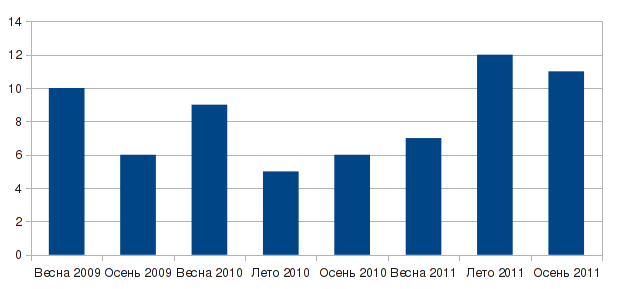
\includegraphics[width=0.8\textwidth]{01-projects.png}
    \caption{Число студенческих проектов по семестрам, 2009 - 2011 гг.}
    \label{projects}
  \end{center}
\end{figure}

Интересно также то, что в осенние семестры студенческие проекты оказывались менее популярны, чем в весенние. Это объясняется в большей степени тем, что весной у второкурсников происходит распределение по кафедрам, а активным участием в студпроекте можно заработать рекомендацию на интересующую кафедру. 

Большое количество летних школ по программированию в 2011 году объясняется тем, что в организации этого мероприятия приняло участие сразу несколько компаний. Так, помимо традиционных проектов от ЗАО ``Ланит-Терком'', работа проводилась еще в двух направлениях: разработка дружественных пользовательских интерфейсов (при поддержке лаборатории Sprint и компании Intel), системному программированию и компьютерной безопасности (при поддержке компаний Digital Design, EMC, Лаборатория Касперского, ЦентрИнформ). В этом году три этих направления были объединены в единую школу системного программирования при кафедре системного программирования СПбГУ. Однако, де-факто они были в значительной степени обособлены. В дальнейшем планируется теснее интегрировать между собой эти и другие летние IT-мероприятия для студентов, проводимые в СПбГУ.

\section{Обзор студенческих проектов 2011 года}

Остановимся подробнее на проектах, проведенных кафедрой системного программирования СПбГУ в 2011 году при сотрудничестве с ЗАО ``Ланит-Терком''. Большая часть из них была нацелена на изучение популярных сейчас мобильных и Интернет-технологий.

Так, несколько проектов было посвящено мобильной платформе Android. В рамках проекта ``Цена денег'' был разработан виджет, позволяющий отображать текущую ситуацию на различных рынках: российском валютном рынке, рынке цветных металлов и т.п. Другой проект ``Android-GeoCacheing.su'' был посвящен взаимодействию мобильных приложений с Интернет-сервисами, а также программному использованию GPS-приемника и магнитного компаса для реализации навигационных приложений. Разработка в этих проектах происходила на языке Java. 

Проект ``iPhoneCF'' также был направлен на разработку ПО в области мобильных платформ. Его целью была создание инструмента для построения распределенных систем, работающих в операционной системе iPhone. Помимо собственно технологических вопросов (знакомство с операционными системами Mac OS, iPhone OS, а также языком Objective C и средой разработки Xcode) в данном проекте много внимания уделялось организации процесса разработки: работа велась в соответствии с ``гибкой'' методологией Scrum. В дальнейшем проект был продолжен под названием ``NeuronIOS'' и был посвящен созданию среды для реализации приложений для операционной системы iPhone, использующих аппарат нейронных сетей для обработки и анализа данных.

Проект ``Basis'' ставил своей целью создание среды для разработки php-приложений. Подобный инструментарий должен минимизировать затраты php-программиста на написание типовых управляющих элементов интерфейса и функций, а также предоставить разработчику каркас приложения, в котором разделена логика по обработке запросов, по работе с базой данных и т.п. Работы велись на языке PHP5 с использованием технологии AJAX.

Проект ``News Aggregating Agent'' предполагал создание приложения для социальных сетей, выполняющих просмотр собираемых с различных Интернет-источников новостей с возможностью фильтрации (по каналу, теме и/или дате). В рамках данного проекта студенты знакомились с программными интерфейсами ведущих социальных сетей и учились создавать Web-приложения на языке haXe.

Проект ``BoardGameMaster'' посвящен другому популярному в наше время типу Интернет-приложений --- многопользовательским онлайн-играм. Задача данного проекта заключалась в разработке Web-сервиса, обеспечивающего возможность реализации любой игры с последовательными действиями игроков (от традиционных шахмат до современных настольных игр). В качестве примера клиентского приложения была разработана электронная версия настольной игры Dominion, разработка которого велась с использованием технологии Flash. Данный студпроект разрабатывался  в течение нескольких семестров.

В рамках проекта ``SUGAR'' студенты занимались созданием приложения для работы с кулинарными рецептами. Данное приложение позволяло по заданному набору продуктов выдать рекомендации, что из них лучше приготовить и как именно, а также подсказывало, что и в каком количестве необходимо дополнительно купить, предоставляя возможность осуществить заказ в Интернет-магазине. Здесь активно использовались технологии компании Miscrosoft --- платформа .NET 3.5-4, Silverlight, SQL Server.

Еще один проект проводился в контексте совместной инициативы ЗАО ``Ланит-Терком'' и кафедры системного программирования под названием DocLine~\cite{docLine1, docLine2, docLine3}. Проект был направлен на освоение студентами одной из самых популярных платформ разработки Java-приложений --- Eclipse, в том числе технологий работы с XML-документами и одной из самых мощных на сегодняшний день платформы для автоматизированного создания графических редакторов --- Eclipse Graphical Modeling Framework (GMF). В качестве области для экспериментов проводилась разработка средства для создания и управления семейством пользовательской документации программного продукта. 
 
Также внимания заслуживают проекты Embox\footnote{Проект Embox, \url{ http://code.google.com/p/embox/}} и QReal~\cite{qreal2, qreal3, qreal}, разрабатываемые как свободное программное обеспечение и традиционно предлагаемые в рамках студенческих проектов и летних школ. 

Проект Embox направлен на создание переносимой  и конфигурируемой операционной системы реального времени для нужд встроенных приложений. Данная система может использоваться на всех стадиях разработки встроенных приложений --- от проектирования аппаратной части до создания функционального ПО. Операционная система  должна запускаться на различных процессорных архитектурах и включать в себя сетевой стек, файловую подсистему, частично поддержан стандарт POSIX и многое другое. Проект ведется уже несколько лет и каждый год привлекает много новых студентов, интересующихся внутренним устройством операционных систем.  

Проект QReal посвящен модельно-ориентированному подходу к разработке ПО, в частности, предметно-ориентированному моделированию --- созданию metaCASE-системы\footnote{MetaCASE-инструментарий --- набор инструментов для создания CASE-систем, \url{http://en.wikipedia.org/wiki/MetaCASE_tool}}. В рамка проекта ведется разработка инструментария, позволяющего быстро создавать новые графические языки и визуальные редакторы для них, а также генераторы кода в различные целевые языки, визуальные отладчики и другие полезные для разработки ПО средства. Студенты знакомятся с устройством визуальных языков, а также принимают активное участие в развитии системы QReal.

\section{Чему и как студенты учатся по время студенческих проектов и летних школ}

Обсудим в деталях, что студенты получают при участии в летних школах и студенческих проектах дополнительно к традиционному университетскому образованию:

\begin{itemize}
 \item знакомство с новыми языками программирования и технологиями;
 \item дополнительная практика программирования в коллективном проекте;
 \item возможность попробовать свои силы в различных областях программной инженерии и выбрать наиболее интересное для себя направление;
 \item непосредственное знакомство с инженерными практиками, применяемыми в промышленных проектах по разработке ПО;
 \item развитие навыков общения в команде;
 \item формирование чувства ответственности за свою работу, знакомство с дисциплиной обязательств.
\end{itemize}

Итак, для студента участие в студенческом проекте прежде всего --- это знакомство с новейшими технологиями программирования и передовыми областями индустрии. Чтобы оставаться конкурентоспособными на рынке, компании по разработке ПО следят за последними тенденциями и новейшими направлениями, критичными для их бизнеса, и стараются поддерживать у своих сотрудников соответствующие компетенции на высоком уровне. При этом чем более новым является тот или иной язык программирования, инструментарий или технология, тем меньше по ним доступно учебных материалов. Таким образом, непосредственное общение с носителями этих знаний из индустрии становится, фактически, единственным достоверным источников информации для студентов, да и для университетских преподавателей.  

Еще одной особенностью проведения студпроектов является то, что студенты вольны сами выбирать проект, в котором они хотят принять участие. При этом очень часто случается так, что изначально каждый студент вступает сразу в несколько проектов, из которых в течение некоторого времени выбирает наиболее интересный для себя (продуктивно работать в нескольких проектах и хорошо учиться практически никогда не получается). Это очень важно, поскольку студенты, особенно на первом-втором курсах, не всегда знают, что они хотят. В такой ситуации для студента было бы идеальным попробовать свои силы в нескольких областях программной инженерии, чтобы впоследствии при трудоустройстве на работу уже иметь сложившееся видение того, чем ему хочется заниматься. В некотором смысле этому способствуют курсовые и дипломные работы, а также производственная преддипломная практика. Однако курсовые работы часто имеют более научную направленность, чем производственную, а производственную практику студент проходит уже в самом конце обучения. 
Наличие разнообразных проектов уже на младших курсах обучения видится нам удачным средством для формирования у студентов кругозора, поэтому мы всячески заинтересованы в расширении спектра наших проектов. 

В студенческих проектах есть возможность непосредственного обучения инженерным практикам, ставшими де-факто обязательной частью повседневной работы промышленного программиста --- средствами тестирования, документирования, конфигурационного управления и др. Так, например, на ``игрушечных'' учебных заданиях, которые предлагаются на лабораторных и практических занятиях в рамках стандартного учебного процесса и которые редко превышают нескольких тысяч строк кода, студенту сложно понять, зачем ему может понадобиться осуществлять ночные сборки и регулярно проводить регрессионное тестирование. Зачем и в каком объеме нужно разрабатывать модульные тесты? Почему в системе отслеживания ошибок (bugtracking system) полезно иметь возможность назначить ошибку конкретному разработчику и уметь связывать ошибку с изменениями в коде, исправляющими эту ошибку? Как зависит организация процесса разработки ПО от выбранной политики создания ветвей (branching policy) в современных системах версионного контроля кода? На эти и многие 
другие актуальные в наше время вопросы сложно ответить, сидя за партой, их нужно постичь на собственном опыте. Только тогда приходит осознание необходимости использования тех или иных инструментальных средств и того, как их нужно правильно применять. И это --- путь формирования производственной культуры. Отсутствие глубокого понимания таких вопросов приводит к тому, что инструменты применяются не вследствие того, что они нужны в данной конкретной ситуации, а потому, что ``так научили'' или ``так принято''~\cite{cargoCult}. Участие в студенческих проектах дает студентам возможность познакомиться с различными инженерными практиками в более реальных условиях, не принимая ничего на веру. 

Стоит также отметить, что часто к нам приходят и студенты со смежных специальностей (иногда даже не IT-профиля), активно стремящиеся познакомиться с промышленным программированием самостоятельно. Не имея даже университетских занятий по программной инженерии, участие в студенческих проектах становится для них существенной подготовкой перед реальной работой в промышленных компаниях.

Еще один важный навык, которому можно обучиться лишь на практике --- умение общаться. Здесь речь идет как о живом общении, так и о культуре производственного сетевого общения.  Очень важно уметь продуктивно работать в команде, в частности, уметь задавать вопросы и прояснять для себя неясные моменты в постановке задачи, а не ``домысливать'' их самому (эта привычка студентов на мат-мехе очень сильна в силу акцента на аналитическом подходе к решению задач, но она приводит к тому, что студенты часто начинают делать что-то совершенно свое, отличное от исходного задания). Также важно уметь рассказать о своей работе самым разным людям --- начальству, товарищам, независимым экспертам (как упоминалось ранее, в конце года проводится презентация результатов работы по каждому студенческому проекту, на которую приглашаются все желающие, и объявления о которой расклеиваются по всему факультету заранее). Внутренние и внешние коммуникации являются важной частью повседневной жизни любого проекта, и этому студентов тоже нужно 
учить. При этом можно прочитать все книги по ораторскому искусству, но публично выступать от этого вряд ли кто-то сможет научиться без реальной практики. Важна также культура производственного сетевого общения (у нас этому начинают учить студентов с первой встречи по проекту): на письма нужно отвечать и делать это оперативно, адекватно заполнять поле с темой письма, не посылать писем только со вложением и с пустым ``телом'' и многое другое. Отсутствие этой, казалось бы, элементарной культуры общения будет не только вносить неприятные моменты в общение между членами команды, но и может сильно испортить внешнюю репутацию компании при общении с заказчиками.

Важной особенностью организации рабочего процесса в промышленных компаниях является дисциплина обязательств~\cite{obyzat}:
\begin{itemize}
 \item готовность работников принимать на себя обязательства перед другими;
 \item четкое определение тех обязательств, которые они на себя берут;
 \item стремление прилагать должные усилия к выполнению своих обязательств;
 \item готовность честно и незамедлительно информировать об угрозах выполнению своих обязательств и т.п.
\end{itemize}
Отсутствие подобной дисциплины является неприемлемым для промышленности. Однако, в университетах традиционно складываются более демократичные порядки --- зачастую считается допустимым опоздать на занятие, многие студенты позволяют себе задерживать результаты по курсовым работам, исчезать и появляться в течение семестра, наивно надеясь все сдать в последний момент или, на крайний случай, в начале следующего семестра и т.п. Проведение студенческих проектов помогает воспитать в студентах чувство ответственности за свою работу, осознание важности не терять связь с руководителем и коллегами, брать на себя обязательства и не подводить своих коллег, следовать общему процессу.

Таким образом, внедрение студенческих проектов в образовательный процесс дает возможность студентам не только повысить свои навыки программирования и владения определенными технологиями, но и на собственном опыте познакомиться с актуальными инженерными практиками. Программная инженерия --- практическая дисциплина, а значит, больш\textit{у}ю роль в формировании профессиональных навыков по данному направлению играет передача опыта, описание типичных ошибок, примеры выполнения реальных проектов и т.п. В связи с этим студенческие проекты видятся нам крайне удачным средством внесения реального практического опыта в классическое университетское образование.


\section{Проект QReal}

Помимо образовательной составляющей студенческие проекты также могут способствовать и научно-исследовательской деятельности. Исследования в области программной инженерии так или иначе подразумевают либо создание нового ПО, либо доработку уже существующего, то есть требуют существенных временн\textit{ы}х затрат на программирование. Организация студенческих проектов по наукоемким темам вовлекает студентов в исследовательскую деятельность, позволяя аспирантам и университетским преподавателям более эффективно продвигать работу в интересующих их направлениях.  

Рассмотрим пример такого студенческого проекта --- проект QReal. 

\subsection{Описание проекта}

Проект QReal развивается силами группы студентов, аспирантов и преподавателей кафедры системного программирования СПбГУ под руководством профессора А.Н.Терехова. Проект стартовал как развитие семейства технологий RTST~\cite{rtst} и REAL~\cite{real}, созданных кафедрой системного программирования СПбГУ и ЗАО ``Ланит-Терком'', и подразумевал доработку графо-графической библиотеки и репозитория CASE-инструмента технологии REAL. Проект развивался в рамках курсовых работ и базировался на набиравшем в то время популярность инструментарии Qt\footnote{Инструментарий для создания кроссплатформенных приложений, \url{http://qt.nokia.com/}}. В ходе работ сформировалась идея о создании на основе полученных наработок нового полноценного CASE-инструмента. Прототип такого инструмента, получившего название QReal, был разработан в рамках трех дипломных проектов в 2007 году. 

Изначально перед участниками проекта ставилась задача создания CASE-инструмента с поддержкой UML 2.0, однако быстро сформировалось осознание того, что необходима технология автоматизированного создания и поддержки новых визуальных языков. В результате фокус проекта стал сдвигаться в сторону предметно-ориентированного моделирования, и в настоящее время ведется разработка инструментария, представляющего собой metaCASE-систему. 

\subsection{QReal как последовательность студенческих проектов}

В отличие от своих предшественников, проектов RTST и REAL, проект QReal является некоммерческим и основной своей целью ставит научные исследования в области модельно-ориентированного подхода к разработке программного обеспечения (MDE, Model-Driven Engineering, модельно-ориентированная разработка ПО). При этом для студентов создаваемый metaCASE-инструментарий представляет интерес как с точки зрения процесса разработки подобных средств программирования, так и является площадкой для экспериментов в области MDE. 

Ежегодно на кафедре системного программирования защищается 4-5 курсовых и дипломных работ, выполненных в рамках проекта QReal~\cite{termPapers}. С 2009 года участники научно-исследовательской группы QReal провели три годовых студенческих проекта и две летние школы, в результате в проекте приняли участие в общей сложности около трех десятков студентов. 

Активное вовлечение студентов в работу над проектами по разработке ПО имеет определенные последствия и требует от руководителей дополнительных организационных действий:
\begin{itemize}
 \item Так как никаких требований к студентам для участия в студпроекте не предъявляется, в проект могут прийти студенты, обладающие весьма слабыми навыками программирования. На обучение этим навыкам руководителю придется тратить дополнительные усилия. 
 \item Чем больше программного кода уже существует на момент входа студента в проект, тем больше времени этому студенту придется потратить, чтобы в нем разобраться.
 \item Студенты фактически не имеют никаких обязательств перед проектом, поэтому могут покинуть его в любое время. Руководитель должен следить за тем, чтобы результаты, получаемые студентами, были в достаточной степени отчуждаемы, чтобы при выходе какого-то участника из проекта его задачи могли бы быть отданы кому-то другому безболезненно.
 \item К возможному уходу участников проекта нужно быть готовым еще и морально. На начальный этап обучения студента может тратиться довольно много усилий, после чего студент может потерять интерес к этому проекту или просто найти себе более интересное занятие (например, почувствовать себя готовым к работе в промышленной компании). 
 \item Студенты участвуют в проектах ради собственного интереса, поэтому могут не захотеть выполнять рутинные, но нужные для проекта задачи. Руководитель должен быть способен мотивировать студентов и построить процесс разработки так, чтобы исправлению ошибок и поддержанию стабильности кода уделялось должное количество времени. 
 \item Большинство студентов, приходящих в студенческий проект, практически не имеют опыта участия в коллективной разработке ПО и не осознают ответственности, которую это участие на них накладывает. Руководитель должен организовать работу так, чтобы возможный простой в работе одного участника не приводил к остановке работы у остальных. 
\end{itemize}
Рассмотрим эти и некоторые другие проблемы подробнее.

Знакомство с проектом, развивающимся на протяжении нескольких лет, может потребовать от студентов значительных временных затрат для знакомства с предметной областью, архитектурой проекта и его исходным кодом. Кроме того, большая часть студентов (особенно младших курсов) может не иметь опыта использования применяемых в проектах технологий и языков программирования, так что часто приходится проводить несколько вводных ознакомительных лекций. Например, в QReal до того, чтобы получить первое задание, связанное с какой-либо доработкой разрабатываемой среды, необходимо решить несколько предварительных ``вводных'' задач. Они позволяют студентам познакомиться с основными концепциями активно используемого в проекте инструментария Qt, изучить работу его графической подсистемы. С учетом того, что работа в студпроектах ведется параллельно с процессом обучения, выполнение вводных заданий может занимать от нескольких недель до нескольких месяцев в зависимости от начального уровня подготовки и усердия студента.

Состав группы разработчиков в таких проектах является непостоянным в силу того, что студенты фактически не имеют формальных обязательств перед проектом, а их собственные интересы часто меняются. Например, студент может покинуть проект, не доведя свою задачу до конца. Если не уделять должного внимания документированию и/или ревью кода, в проекте могут начать появляться участки кода, про которые никто не понимает, как они работают. Эту проблему может решить воплощение в жизнь стратегии коллективного владения кодом~\cite{collectiveOwnership}, когда нет выделенных людей, ответственных за какой-то определенный модуль, а каждый имеет представление об всех (или почти всех) компонентах системы и может при необходимости исправить ошибки или реализовать новую функциональность. Этого можно добиться регулярным проведением ревью студентами кода друг друга, а также введением обязательного документирования создаваемой функциональности, например, на вики проекта и/или прямо в коде с помощью языков документирования типа 
doxygen\footnote{Кроссплатформенная система документирования исходных текстов, \url{www.doxygen.org}} или javadoc\footnote{Генератор документации из комментариев исходного кода на Java, \url{http://www.oracle.com/technetwork/java/javase/documentation/index-jsp-135444.html}}. Анализируя подобные проблемы в проекте QReal, мы пришли к следующему решению --- все изменения в исходные коды проекта вносятся только в ``ветвях'' разработки системы контроля версий. Когда изменения завершены, подается запрос на интеграцию с основной ``веткой'', которая осуществляется только после прохождения ревью нового кода. Зная, что их изменения обязательно будут просмотрены и прокомментированы перед интеграцией в основную ``ветку'', студенты стараются программировать аккуратнее. А участие в ревью кода своих коллег позволяет им учиться на чужих ошибках, пытаясь подобным образом анализировать свои решения в дальнейшем. Если нет возможности сделать ревью частью процесса разработки, его все равно стоит проводить на регулярной основе, 
например, один или два раза в неделю для летних школ и, скажем, раз в 2-3 недели для студенческих проектов в течение семестра.

Стоит отметить, что для поддержания в проекте практики общего владения кодом и руководителям, и студентам приходится тратить довольно много ресурсов. Не имея перед собой четких целей, многие студенты не готовы к этому. Если основной целью студпроекта ставится разработка определенного программного обеспечания как таковая, то гораздо менее затратным подходом будет подробная декомпозиция задач и контроль за их выполнением студентами.  При должном уровне детализации можно исправлять ошибку или реализовывать новую функциональность, даже не представляя, как система работает в целом. Такой подход часто хорошо работает в промышленности, особенно при аутсорсинге, когда группа архитекторов или опытных программистов выдает менее опытным (и часто гораздо менее оплачиваемым) разработчикам задачи, которые те должны реализовать в соответствии с определенными интерфейсами. Однако, на наш взгляд, такой подход не стоит применять для проведения студенческих проектов, поскольку подобная организация процесса разработки не дает 
участникам развивать никаких навыков, кроме программирования. Да и осознание полной картины происходящего в проекте, возможность участвовать в принятии решений, назвать проект ``своим'' куда привлекательнее для молодых специалистов, чем однообразное программирование небольших задач. 

Так как большинство студентов участвуют в студенческих проектах ради получения интересного практического опыта, то вполне ожидаемо, что они хотят заниматься вещами, которые им нравятся, и стараются избегать скучных рутинных задач. В частности, практически все студенты  с больш\textit{и}м энтузиазмом берутся за реализацию новой функциональности и неохотно за поддержку и исправление ошибок в существующем коде. Это вполне объяснимо, поскольку разбираться в чужом коде сложно и может потребовать большого количества ресурсов, при этом не принося видимого результата быстро. Этим же объясняется и то, что, получив новую задачу, большинство студентов начинают ее решать ``с нуля'', при том, что либо в этом же проекте, либо где-то в общем доступе есть информация или даже реализация похожей задачи, которую можно проанализировать или взять за основу. Решать эту проблему можно разными способами, например, повышением культуры программирования в проекте, внедрением процесса разработки, близкого к промышленным и т.п. Например,
 в проекте QReal в последнее время исправление открытых ошибок является обязательным видом деятельности для каждого участника. Более того, первыми задачами, которые получают приходящие в проект студенты, является как раз исправление существующих ошибок. Со временем в любом проекте накапливается набор открытых ошибок, которые с точки зрения опытного разработчика исправляются тривиальным образом. Все понимают, что исправлять их нужно, однако участники проекта чаще всего не спешат этого делать, отдавая предпочтение более интересным задачам. По нашему опыту, исправление таких ошибок идеально подходит для введения в проект новых участников, поскольку позволяет им:
\begin{itemize}
 \item в деталях познакомиться с частью исходного кода проекта. В большинстве случаев это будет небольшой по объему участок кода, с которым даже совсем не знакомый с проектом студент справится за разумное время;
 \item привыкнуть к стилю оформления кода и принятому в проекте процессу разработки;
 \item наглядно увидеть результат своей работы, что может сильно поднять уровень заинтересованности студента.
\end{itemize}
Возводить исправление ошибок в ранг обязательной деятельности важно еще и потому, что стадия развития и поддержки существующего кода присутствует в жизненном цикле любого проекта. Для многих студентов младших курсов это может быть неочевидно. В то же время, если перед начинающими участниками ставить задачи, которые, например, будут требовать длительного по времени этапа исследования или программирования (например, серьезный рефакторинг), то студент может просто потерять интерес к выполняемой работе, потерявшись в деталях.

Также важным является возможность для студентов наблюдать динамику развития своего проекта. Например, в стартующих ``с нуля'' небольших проектах (объемом работ в несколько человеко-месяцев) участники проходят весь путь от идеи и до выпуска работающих версий. Нередки ситуации, когда еще неделю назад проект представлял собой набор разрозненных компонент, а через какое-то время они начинают объединяться вместе и представлять собой уже работающее приложение с нетривиальной функциональностью. В таких проектах каждое действие студентов приносит ощутимый результат, поэтому их мотивация повышается. В крупных проектах этого тоже можно добиться, но немного сложнее. Например, в QReal мы стараемся давать студентам задачи, выполнение которых приведет к изменениям в графическом интерфейсе разрабатываемого ПО, добавит новую функциональность, исправит надоедливую, бросающуюся в глаза ошибку или сделает еще что-то заметное. Тогда студентам не будет казаться, что их работа теряется на общем фоне. Если подобные задачи требуют 
большого объема работы, можно объединять студентов в подгруппы.

Особую специфику может добавить участие в проекте, разрабатываемом как свободное программное обеспечение (СПО)~\cite{saratov}. В частности, чувство владения (``feeling of ownership'') кодом продукта у студентов также повышает личную ответственность за реализуемую ими функциональность, что помогает не делать поспешных и необдуманных решений. Стоит отметить, что вначале некоторых студентов может испугать такая открытость и они будут бояться выкладывать свои изменения в публичный доступ. Однако, как показывает практика, в дальнейшем студенты привыкают к концепции открытого ПО вплоть до того, что начинают хвастаться своими успехами перед одногруппниками.

Также возможен подход, когда в студенческом проекте ведется работа над уже существующим открытым проектом (по аналогии с Google Summer of Code~\cite{google}), желательно популярным в своей области. Автоматически снимая вопрос о мотивации, это позволит студентам получить уникальный опыт работы в интернациональной команде опытных разработчиков. Стоит отметить, что для студентов участие в подобных проектах может быть осложнено из-за языкового барьера, в таком случае руководителю нужно быть хорошо знакомым с разрабатываемым проектом и брать часть коммуникаций с основной командой разработчиков на себя. Будет идеально, если руководитель сам будет одним из разработчиков этого продукта. Это позволит более адекватно руководить студентами, выдавая им задачи и координируя их общение с остальными членами команды. Подобный подход кажется нам очень интересным, однако на данный момент опыт проведения подобных студенческих проектов у нас отсутствует.

Начиная с третьего курса студенты кафедры системного программирования СПбГУ выполняют курсовые работы по интересующим их направлениям под руководством преподавателей кафедры. Для студентов младших курсов участие в струденческом проекте или летней школе может быть хорошей подготовкой к написанию курсовой работы, как дисциплинируя студента, так и давая ему возможность получить опыт и повысить свои навыки программирования для решения других задач. Более того, в проекте QReal были случаи, когда по результатам, полученным в рамках студпроектов или летних школ, защищались курсовые работы и делались доклады на студенческих конференциях.

Как отмечалось выше, проведение студенческих проектов и летних школ зависит от множества факторов, начиная от загруженности и уровня подготовки руководителя, числа и квалификации участвующих в проекте студентов и заканчивая степенью самостоятельности участников или даже тем, были ли знакомы студенты друг с другом до участия в проекте. В результате получается ситуация, когда практически невозможно провести два совершенно одинаковых студенческих проекта даже по одной и той же теме --- каждый будет чем-то отличаться от всех остальных. Однако, приведенные выше проблемы так или иначе являются типичными для большинства проектов, а значит, каждому руководителю нужно быть готовым к их решению.

\subsection{Летняя школа в 2011 году}

В 2011 году студенческий проект в рамках QReal был посвящен созданию QReal:Robots --- средства визуального программирования роботов Lego Mindstorms NXT 2.0\footnote{Робототехнический конструктор Lego Mindstorms NXT 2.0, \url{mindstorms.lego.com}}. 

В настоящее время наблюдается активный рост использования робототехнических конструкторов в школах как средств обучения программированию и робототехнике~\cite{filippov}.  Использование реального исполнителя для демонстрации работы внедрялось в образовательный процесс еще с языка Logo\footnote{Язык Logo, \url{http://tiny.cc/wiki-logo}}, разработанного Сеймуром Пейпертом в 60-х годах прошлого века. Современный уровень развития вычислительной техники позволяет создать недорогие устройства как исполняющие внутреннюю программу, так и управляемые по беспроводной связи с персонального компьютера. Такие устройства уже существуют, и робототехнические конструкторы на базе соответствующих контроллеров уже активно внедряются в школьное образование. Одним из самых популярных конструкторов является Lego Mindstorms NXT 2.0. Однако, существующие средства программирования таких устройств во многом не устраивают школьных учителей. В частности, некоторые из существующих средств недостаточно функциональны, другие не позволяет 
наглядно отлаживать создаваемые программы, не имеют возможностей перехода от графического представления программы к текстовому, не до конца переведны на русский язык, а также зачастую небесплатны.

При сотрудничестве с кафедрой теоретической кибернетики СПбГУ и ФМЛ №239 г. Санкт-Петербурга было решено разработать отечественное визуальное средство программирования роботов Lego Mindstorms NXT 2.0 --- QReal:Robots. Первым этапом разработки стала инструментальная среда, основанная на диаграммном подходе к программированию. Используя пиктограммы функциональных и логических блоков и соединяя их связями-переходами (см. рис.~\ref{qreal-robots}), программист задает алгоритм поведения робота, который потом исполняется на реальном устройстве (подробнее про проект QReal:Robots см. в~\cite{robots}).

\begin{figure} [ht]
  \begin{center}
    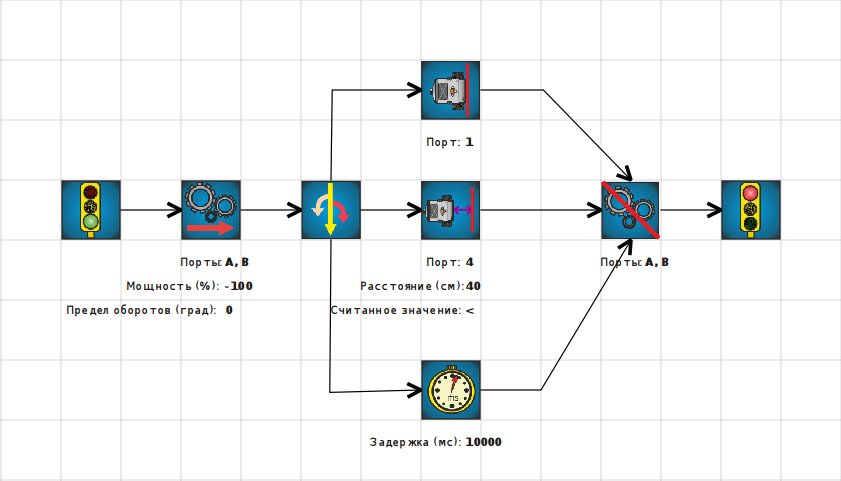
\includegraphics[width=0.9\textwidth]{02-qreal-robots.png}
    \caption{Пример программы в QReal:Robots}
    \label{qreal-robots}
  \end{center}
\end{figure}

Проект стартовал в январе 2011 года, так что к началу летней школы уже существовал прототип с реализованными базовыми операциями. Важной особенностью именно этой школы стало фактическое наличие у создаваемого продукта внешнего заказчика и жестких сроков. В качестве заказчиков выступали заинтересованные в этом программном продукте учителя, которым посредством выступления на тематических конференциях было анонсировано о выпуске бета-версии продукта к началу нового учебного года, т.е. формально через некоторое время после завершения летней школы. Это добавило участникам летней школы дополнительной мотивации, поскольку они понимали, что создаваемый ими продукт --- это не учебная разработка, он действительно нужен. Осознание этого факта позволяло студентам более ответственно относиться к ставившимся перед ними задачам. 

Стоит отметить, что в случае, когда фактический заказчик отсутствует, его роль может взять на себя руководитель проекта. Однако, это может вызвать дополнительные сложности, поскольку руководителю придется совмещать роли, интересы которых в проекте традиционно конфликтуют --- заказчик хочет как можно больше функциональности за меньший объем ресурсов, а менеджер проекта пытается сократить объем планируемой функциональности в пользу качества и стабильности проекта в целом. Если же руководитель проекта берет на себя только роль заказчика, управление проектом и организация команды перекладывается на плечи студентов, что в отсутствие у них подобного опыта может стать непосильной задачей.

В рассматриваемой летней школе участвовало восемь студентов, из них только для троих проект был новым. Остальные пятеро к тому моменту уже участвовали в студенческом проекте и летней школе 2010 года. Новоприбывшие участники обладали довольно хорошей подготовкой, поэтому быстро разобрались с поставленными перед ними задачами. Это позволило свести ``вводную'' фазу летней школы к минимуму и больше времени посвятить разработке новой функциональности и исправлению ошибок. 

До начала летней школы в QReal:Robots существовал только один способ исполнения создаваемых программ на роботе --- пошаговая интерпретация диаграмм и синхронная передача команд, соответствующих исполняемым блокам, в робота по Bluetooth\footnote{Беспроводной протокол для организации персональных сетей, \url{www.bluetooth.org}}. Данный подход обеспечивал наглядность и позволял оперативно отлаживать разрабатываемые алгориты, однако, обмен данными по протоколу Bluetooth вносил довольно существенную задержку в общение с роботом. Это делало невозможным адекватное выполнение весьма широкого класса программ, требующих реагирования в реальном времени в зависимости от показаний датчиков робота --- например, объезд препятствия. Для решения этой проблемы была поставлена задача реализовать в QReal:Robots возможность получать по создаваемым диаграммам бинарный код соответствующей программы, передавать его на робота и запускать там на автономное исполнение.

Решение данной задачи подразумевало работу сразу по нескольким направлениям. Во-первых, нужно было выбрать целевую платформу для генерации. Существует несколько операционных систем, способных запускаться и работать на роботах Lego Mindstorms NXT 2.0, студенты рассмотрели самые популярные, проанализировали их достоинства и недостатки и выбрали наиболее подходящую для наших целей. После того, как целевая платформа была выбрана, был создан генератор кода (в нашем случае генерировались программы на Си-подобом языке с использованием прикладного интерфейса, предоставляемого платформой), средства для удобного отображения генерируемого кода в QReal:Robots, скрипты для сборки получаемых программ и средства для передачи получаемых бинарных файлов на робота по протоколу USB. Также был создан инсталлятор, реализована поддержка некоторых дополнительных типов функциональных блоков на диаграммах, реализован более функциональный вариант окна настроек QReal:Robots и панели настроек блоков и многое другое.

Кроме реализации новой функциональности много времени уделялось исправлению открытых ошибок (за три недели летней школы было исправлено около 20 ошибок), стабилизации и рефакторингу имеющегося кода. Стоит заметить, что этот процесс для студенческих проектов совершенно необходим, в особенности для проектов, длящихся более одного года. Причин для этого несколько --- во-первых, в образовательных целях, а во-вторых, как показывает наш опыт, чтобы код, разрабатываемый студентами, оставался ``чистым'', читаемым и сопровождаемым, за ним нужно следить более опытным разработчикам. Так, например, часть функциональности, реализованной в летней школе по QReal:Robots, доводилась до финального состояния вплоть до новогодних каникул уже опытными участниками проекта. При отсутствии должного внимания качество кода начинает падать, что потом может вылиться в то, что студентам будет просто не интересно продолжать разрабатывать систему дальше.

\section{Заключение}

Традиционное университетское образование направлено в первую очередь не на получение практических навыков, а на формирование особого образа мышления студентов --- умения искать и анализировать информацию, находить новые пути решения задач. Для обучения по специальностям, связанным с программной инженерией, это имеет свои плюсы и минусы: с одной стороны, выпускник классического университета получает фундаментальную теоретическую подготовку для работы в своей области --- знает основные алгоритмы и структуры данных, языки программирования, технологии и подходы к разработке ПО и т.д. С другой стороны, налицо явный недостаток практических навыков, и это хорошо понимают в промышленных компаниях --- к большинству из открытых в индустрии вакансий ставится требованием наличие нескольких лет опыта работы по специальности. Осознавая это, студенты IT-специальностей, начиная с третьего-четвертого курса, уже пытаются устраиваться на работу стажерами. Но очень часто это приводит тому, что у них остается очень мало времени 
на учебу. В результате уровень получаемого выпускниками образования снижается.

Наш опыт проведения студенческих проектов и летних школ по программированию на базе кафедры системного программирования СПбГУ показывает, что для студентов опыт участия в них крайне полезен. Участвуя в таких мероприятиях, студенты не только повышают свои навыки программирования, но и знакомятся с полезными инженерными практиками, которые помогут им по завершении обучения быть полноценными специалистами в области программной инженерии. Однако, очень многое зависит от организации подобных проектов. Так, руководитель должен быть способен увлечь участников проекта своей идеей, донести ее до студентов в понятном и привлекательном виде. На руководителя проекта ложатся все действия по организации команды и обеспечению условий продуктивной работы, по организации коммуникаций в проекте, построению процесса разработки и многое другое. Все это требует существенных усилий и временн\textit{ы}х затрат, и к этому нужно быть готовым. При этом руководитель проекта должен не только сам быть опытным разработчиком ПО, но и 
уметь делиться своими знаниями со студентами (что среди технических специалистов далеко не настолько распространенный навык, насколько хотелось бы). 

Исходя из нашего опыта, в организационном аспекте студенческие проекты сильно отличаются от промышленных коммерческих проектов. Так, например, очень многое зависит от того, что студенты участвуют в подобных проектах только ради собственного интереса, тратя на это только часть свободного времени. Также значительное количество времени в начале проекта тратится на обучение студентов используемым языкам и технологиям, на введение в предметную область. Или, например, часто случается так, что, повысив свои навыки до определенного уровня и начав действительно вносить нетривиальный вклад в развитие проекта, студент либо переходит в другой студпроект, либо устраивается на работу в промышленную компанию, сводя свое участие в студенческом проекте к минимуму. Чтобы двигаться вперед, руководителю нужно прикладывать больше усилий для фиксирования текущих результатов (например, в виде проектной документации) и сохранения стабильности разрабатываемого ПО. 

Однако, как показывает наш опыт, при должных усилиях к организации процесса разработки и коммуникаций в проекте студенческие проекты и летние школы по программированию являются очень удачным средством как для обучения студентов программной инженерии, так и для организации научных исследований в этой области. 

\begin{thebibliography}{9001}

  \bibitem{robots} \emph{Брыксин Т.А., Литвинов Ю.В.} Среда визуального программирования роботов QReal:Robots // Материалы международной конференции ``Информационные технологии в образовании и науке''. Самара. 2011. С. 332--334.
  
  \bibitem{gagarsky} \emph{Гагарский Р.К.} Программа подготовки специалистов в IT-компании // Системное программирование. Вып. 3. СПб.: Изд-во СПбГУ. 2008. С. 141--156.
  
  \bibitem{termPapers} Курсовые и дипломные работы, защищенные на кафедре системного программирования СПбГУ по проекту QReal. \url{http://tiny.cc/qreal}

  \bibitem{apkit} Квалификационные требования (профессиональный стандарт) в области информационных технологий по специальности ``Программист'', http://apkit.ru/files/programer.doc
  
  \bibitem{saratov} \emph{Кириленко Я.А.} Разработка свободного программного обеспечения для школ как средство обучения программной инженерии // Материалы IX Всероссийской конференции ``Преподавание информационных технологий в Российской Федерации''. Саратов. 2011.
  
  \bibitem{docLine1} \emph{Кознов Д.В., Романовский К.Ю.}  DocLine: метод разработки документации семейства программных продуктов. Программирование. 2008. № 4. С. 1--13.

  \bibitem{docLine2} \emph{Кознов Д.В., Романовский К.Ю.} Автоматизированный рефакторинг документации семейств программных продуктов // Системное программирование. Вып. 4: Сб. статей / Под ред. А.Н.Терехова, Д.Ю.Булычева. СПб.: Изд-во СПбГУ. 2009. С. 127--149.
  
  \bibitem{obyzat} \emph{Кознов Д.В.} Введение в программную инженерию, часть I. Учебное пособие. СПбГУ. 2005. 41 с. 

  \bibitem{collectiveOwnership} Коллективное владение кодом в методологии XP. \url{http://www.extremeprogramming.org/rules/collective.html}
  
  \bibitem{qreal2} \emph{Кузенкова А.С., Дерипаска А.О., Таран К.С., Подкопаев А.В., Литвинов Ю.В., Брыксин Т.А.} Средства быстрой разработки предметно-ориентированных решений в metaCASE-средстве QReal // Научно-технические ведомости СПбГПУ, Информатика, телекоммуникации, управление. Вып. 4 (128). СПб.: Изд-во Политехнического Университета. 2011. С. 142--145.

  \bibitem{qreal3}\emph{Осечкина М.С., Брыксин Т.А., Литвинов Ю.В., Кириленко Я.М.} Поддержка жестов мышью в мета-CASE-системах // Системное программирование. Вып. 5: Сб. статей / Под ред. А.Н.Терехова, Д.Ю.Булычева.  СПб.: Изд-во СПбГУ, 2010. С. 52--75.

  \bibitem{curriculum} Рекоммендациях по преподаванию программной инженерии и информатики в университетах, \url{http://www.intuit.ru/research/se2004.pdf}  

  \bibitem{rtst} \emph{Парфенов В.В., Терехов А.Н.} RTST --- технология программирования встроенных систем реального времени. // Системная информатика. Новосибирск. 1997. N5. C. 228--256.
  
  \bibitem{docLine3}\emph{Смирнов М.Н., Кознов Д. В., Дорохов В. А., Романовский К.Ю.} Программная среда WebMLDoc для автоматизированного отслеживания изменений в пользовательской документации Web-приложений // Сб. Системное программирование./ Вып. 5, под ред. А.Н.Терехова и Д.Ю.Булычева. СПб.: Изд. СПбГУ. 2010. C. 32--51.
  
  \bibitem{schoolList} Список  евпропейских летних школ с 1998 по 2011 по IT, \url{http://user.it.uu.se/~bengt/Info/summer-schools.shtml}

  \bibitem{terekhov1}\emph{Терехов А.Н.} Что такое программная инженерия // Программная инженерия, 2010, Вып. 1. Изд-во ``Новые технологии''. С. 40--45.

  \bibitem{qreal} \emph{Терехов А.Н., Брыксин Т.А., Литвинов Ю.В., Смирнов К.К., Никандров  Г.А., Иванов В.Ю., Такун Е.И.} Архитектура среды визуального  моделирования QReal // Системное программирование. Вып. 4: Сб. статей  / Под ред. А.Н.Терехова, Д.Ю.Булычева. 2009. С. 171--196.

  \bibitem{terekhov2}\emph{Терехов А.А., Терехов А.Н.} Computing Curricula: Software Engineering и российское образование. // Открытые системы, 2006, № 8. Изд-во ``Открытые системы''. С. 61--66.

  \bibitem{terekhov3}\emph{Терехов А.Н.} Вспоминая о статье ``Как готовить системных программистов'' // Компьютерные инструменты в образовании, 2007, №4. С. 3--12.

  \bibitem{real} \emph{Терехов А.Н., Романовский К.Ю., Кознов Д.В., Долгов П.С., Иванов А.Н.} REAL: методология и CASE-средство для разработки систем реального времени и информационных cистем, Программирование, 1999, № 5. C. 44--52.

  \bibitem{filippov} \emph{Филиппов С.А.} Робототехника для детей и родителей. Наука. 2011. 264 с.

  \bibitem{google} Google Summer of Code, \url{http://code.google.com/intl/ru-RU/soc/}

  \bibitem{swebok} Guide to the Software Engineering Body of Knowledge (SWEBOK), \url{http://www.computer.org/portal/web/swebok}
  
  \bibitem{langList} HOPL: an Interactive Roster of Programming Languages,  \url{http://hopl.murdoch.edu.au/}
  
  \bibitem{cargoCult} Steve McConnell, Cargo Cult Software Engineering. From the Editor, IEEE Software, March/April 2000, \url{http://stevemcconnell.com/ieeesoftware/eic10.htm}


\end{thebibliography}

\end{document}
